% !TEX program = lualatex
% Generated by new_lecture_note.sh
\documentclass[11pt]{article}

\usepackage{fontspec}
\usepackage{microtype}
\usepackage{mathtools,amssymb,amsfonts,amsthm,bm}
\usepackage{tikz}
\usepackage{enumitem}
\usepackage{xcolor}
\usepackage{booktabs,array,xcolor}
\usepackage{geometry,fancyhdr,setspace}
\usepackage[hidelinks]{hyperref}
\usepackage[nameinlink,noabbrev]{cleveref}

\geometry{margin=1in,headheight=15pt}
\setstretch{1.12}
\setlength{\parindent}{0pt}
\setlength{\parskip}{0.55em plus 0.12em minus 0.08em}
\setlength{\abovedisplayskip}{0.8em plus 0.2em minus 0.1em}
\setlength{\belowdisplayskip}{0.8em plus 0.2em minus 0.1em}
\allowdisplaybreaks[3]
\setlist{leftmargin=*,topsep=0.35em,itemsep=0.15em,parsep=0pt}

% ---------- Metadata ----------
\newcommand{\studentname}{Keshav Ramamurthy}
\newcommand{\coursename}{Math 118}
\newcommand{\lecturenumber}{02}
\newcommand{\lecturetitle}{Lecture 02}
\newcommand{\lecturedate}{\today}

% ---------- Reusable notation ----------
\newcommand{\N}{\mathbb{N}}
\newcommand{\Z}{\mathbb{Z}}
\newcommand{\Q}{\mathbb{Q}}
\newcommand{\R}{\mathbb{R}}
\newcommand{\C}{\mathbb{C}}
\newcommand{\F}{\mathbb{F}}
\newcommand{\K}{\mathbb{K}}
\newcommand{\E}{\mathbb{E}}
\newcommand{\Prob}{\mathbb{P}}
\newcommand{\1}{\mathbf{1}}
\newcommand{\eps}{\varepsilon}
\newcommand{\dd}{\,\mathrm{d}}
\newcommand{\abs}[1]{\left\lvert#1\right\rvert}
\newcommand{\norm}[1]{\left\lVert#1\right\rVert}
\newcommand{\ip}[2]{\left\langle#1,#2\right\rangle}
\newcommand{\set}[1]{\left\{#1\right\}}
\newcommand{\given}{\,\middle\vert\,}
\newcommand{\indep}{\perp\!\!\!\perp}
\newcommand{\lto}{\longrightarrow}
\newcommand{\deriv}[2]{\frac{\mathrm{d}#1}{\mathrm{d}#2}}
\newcommand{\pderiv}[2]{\frac{\partial#1}{\partial#2}}
\DeclareMathOperator{\Aut}{Aut}
\DeclareMathOperator{\Hom}{Hom}
\DeclareMathOperator{\Ker}{ker}
\DeclareMathOperator{\im}{im}
\DeclareMathOperator{\rank}{rank}
\DeclareMathOperator{\nullity}{nullity}
\DeclareMathOperator{\Span}{span}
\DeclareMathOperator{\Var}{Var}
\DeclareMathOperator{\Cov}{Cov}

% ---------- Note environments ----------
\newtheoremstyle{notestyle}{0.7em}{0.7em}{\itshape}{}{}{\bfseries}{.5em}{}
\theoremstyle{notestyle}
\newtheorem{theorem}{Theorem}[section]
\newtheorem{lemma}[theorem]{Lemma}
\newtheorem{proposition}[theorem]{Proposition}
\newtheorem{corollary}[theorem]{Corollary}
\theoremstyle{definition}
\newtheorem{definition}[theorem]{Definition}
\newtheorem{example}[theorem]{Example}
\newtheorem{remark}[theorem]{Remark}
\newenvironment{claim}{\par\noindent\textbf{Claim.}\ }{\par}
\newenvironment{idea}{\par\noindent\textit{Idea.}\ }{\par}
\newenvironment{proofsketch}{\par\noindent\textbf{Proof sketch.}\ }{\par}

% ---------- Header ----------
\pagestyle{fancy}
\fancyhf{}
\fancyhead[L]{\coursename}
\fancyhead[C]{\lecturetitle}
\fancyhead[R]{\studentname}
\fancyfoot[C]{\thepage}

\title{\vspace{-1.5em}\textbf{\coursename -- \lecturetitle}}
\author{\studentname}
\date{\lecturedate}

\begin{document}
\maketitle

\section{Norms, Inner Products, Cauchy, etc}
\begin{definition}[norm]
\label{def:label}
A norm on a vector space V is a mapping $||. || : V \rightarrow [0, \infty).$
with properties 
\begin{itemize}
    \item Triangle Inequality: $||u + v|| \le ||u|| + ||v||.$
    \item Homogeneity $||\alpha u|| = |\alpha| ||u||$
    \item Positive Definiteness. $||u|| = 0 \iff u = 0$
    \item Distance from u and v is $||u-v||$
\end{itemize}
\end{definition}
\subsection{Norms on $R^n$ or $C^n$}
\begin{itemize}
    \item One-norm: $||x||_{1} = \sum_{k=1}^{n} |x_k|$
    \item  Two-norm: $||x||_{2} = \sqrt{\sum_{k=1}^{n}(x_k)^2}$
    \item Max-norm: $||x||_{\infty} = \max_{k \le n} |x_k|$
\end{itemize}
\begin{definition}[Unit Ball]
\label{def:label}
$B = \{x \in V : ||x|| \le 1\}$
\end{definition}
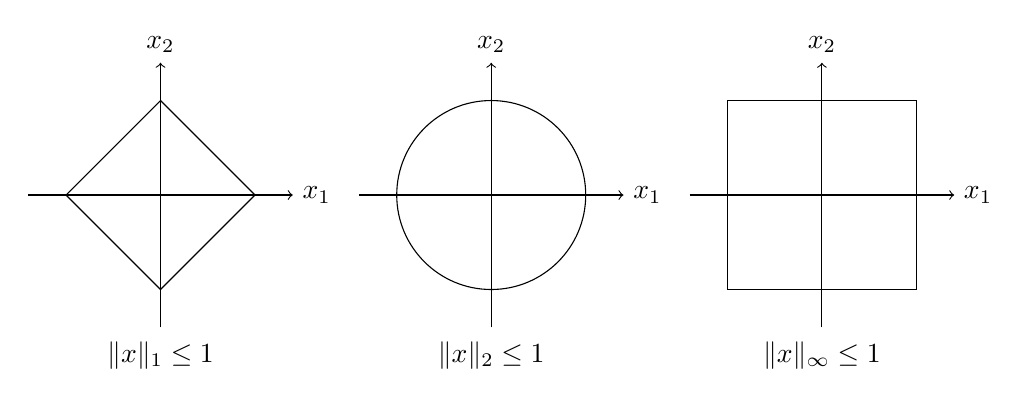
\begin{tikzpicture}[scale=1.2]
    % 1-norm
    \draw[->] (-1.4,0) -- (1.4,0) node[right] {$x_1$};
    \draw[->] (0,-1.4) -- (0,1.4) node[above] {$x_2$};
    \draw (1,0) -- (0,1) -- (-1,0) -- (0,-1) -- cycle;
    \node at (0,-1.7) {$\|x\|_1 \leq 1$};

    % 2-norm
    \begin{scope}[xshift=3.5cm]
        \draw[->] (-1.4,0) -- (1.4,0) node[right] {$x_1$};
        \draw[->] (0,-1.4) -- (0,1.4) node[above] {$x_2$};
        \draw (0,0) circle (1);
        \node at (0,-1.7) {$\|x\|_2 \leq 1$};
    \end{scope}

    % infinity-norm
    \begin{scope}[xshift=7cm]
        \draw[->] (-1.4,0) -- (1.4,0) node[right] {$x_1$};
        \draw[->] (0,-1.4) -- (0,1.4) node[above] {$x_2$};
        \draw (-1,-1) rectangle (1,1);
        \node at (0,-1.7) {$\|x\|_\infty \leq 1$};
    \end{scope}
\end{tikzpicture}
\par For any $ x\in \mathbb{C}^{n}$, we have $$||x||_{\infty} \le ||x||_2 \le ||x||_1$$
because $$|x||_{\infty} = \sqrt{\max_{k} |x_k|^2} \le \sqrt{\sum_{k} |x_k|^2}$$
% \textit{Write the one-sentence point of today's lecture here.}
\[
x =
\begin{pmatrix}
x_1\\
x_2\\
\vdots\\
x_n
\end{pmatrix},
\qquad
e_j =
\begin{pmatrix}
0\\
\vdots\\
0\\
1\\
0\\
\vdots\\
0
\end{pmatrix}
\quad
\text{($1$ in the $j$th slot)}
\]
where $(e_j)_i = S_{ij} =
\begin{cases}
1, & i=j,\\
0, & i\ne j.
\end{cases}$
\par So we can rewrite $$||x||_2 = ||x_1e_1 + x_2 e_2 + \cdots + x_n e_n||_2$$
By the triangle inequality we have 
$$ ||x_1e_1 + x_2 e_2 + \cdots + x_n e_n||_2 \le ||x_1e_1||_2 + ||x_2e_2||_2 + \cdots +
||x_ne_n||_2$$
$$||x_1e_1||_2
+  \cdots + ||x_ne_n||_2 = |x_1|||e_1||_2 + |x_2|||e_2||_2 + \cdots + |x_n| ||e_n||_2$$
Notice by definition of $e_i$ its two norm would be 1, so this is just $\sum_{i} |x_k| =
||x||_1$
\begin{remark}[Unit Balls Nested in the opposite direction]
\label{rem:label}
We have $$B_1 \subseteq B_2 \subseteq B_{\infty}$$

\[
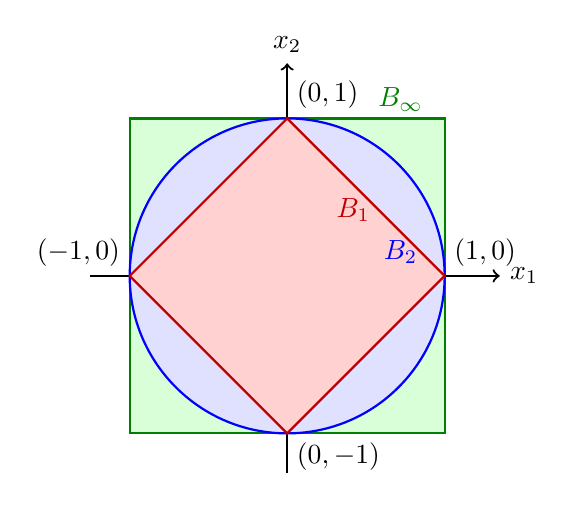
\begin{tikzpicture}[scale=2]

    % Axes
    \draw[->, thick] (-1.25,0) -- (1.35,0) node[right] {$x_1$};
    \draw[->, thick] (0,-1.25) -- (0,1.35) node[above] {$x_2$};

    % B_infinity
    \fill[green!15] (-1,-1) rectangle (1,1);
    \draw[thick, green!50!black] (-1,-1) rectangle (1,1);

    % B_2
    \fill[blue!12] (0,0) circle (1);
    \draw[thick, blue] (0,0) circle (1);

    % B_1
    \fill[red!18] 
        (1,0) -- (0,1) -- (-1,0) -- (0,-1) -- cycle;
    \draw[thick, red!75!black]
        (1,0) -- (0,1) -- (-1,0) -- (0,-1) -- cycle;

    % Coordinate labels
    \node[above right] at (1,0) {$(1,0)$};
    \node[above left] at (-1,0) {$(-1,0)$};
    \node[above right] at (0,1) {$(0,1)$};
    \node[below right] at (0,-1) {$(0,-1)$};

    % Ball labels
    \node[red!75!black] at (0.42,0.42) {$B_1$};
    \node[blue] at (0.72,0.15) {$B_2$};
    \node[green!50!black] at (0.72,1.12) {$B_\infty$};

\end{tikzpicture}
\]
\par if $x \in B$, then $||x||_1 \le 1$ so $$||x||_2 \le ||x||_1 \le 1$$
\end{remark}
\section{Inner Products}
% An inner product is a mapping $\langle ., . \rangle : V x V \rightarrow \mathbb{C}$ such
% that 
An inner product is a mapping
\(
\langle \cdot,\cdot\rangle : V\times V \to \mathbb{C}
\)
such that
\begin{enumerate}
    \item $\langle u, u\rangle > u \text{ if } x \ne 0$
    \item $\langle v, u\rangle = \overline{\langle u, v \rangle}$
    \item $\langle \alpha u, v\rangle = \alpha \langle u, v \rangle.$
    \item $\langle u + v, w\rangle = \langle u, w\rangle + \langle v, w\rangle$
    \item 3 implies that $\langle 0, v\rangle = 0$
    \item 2 and 3 imply that $\langle u, \alpha v\rangle = \overline{\alpha}\langle u,
        v\rangle$ 
    % \item $(\langle, .)$ is a sesquilinear form) $$\overline{\alphakj
    \item 2 and 4 imply that $\langle w, u + v \rangle = \langle w, u \rangle + \langle
        w, v\rangle$
\end{enumerate}
Geometrically: $$\langle u, v \rangle = ||u|| \cdot ||v|| \cdot \cos \theta$$
$$|| \alpha u || = \sqrt{\langle \alpha u, \alpha u \rangle } = \sqrt{\alpha
\overline{\alpha} \langle u, u\rangle} = |\alpha|\sqrt{\langle u, u \rangle}$$
In physics,usually the innter product is defined to be by linear in y. 
\begin{theorem}[Cauchy--Schwarz]
\label{thm:cauchy-schwarz}
For all $u, v \in V$:
$$|\langle u, v\rangle | \le ||u ||  \cdot ||v||$$
The proof -- along with Pythagoras and the corollaries (triangle inequality, induced
norm, angles) -- is written out in the dedicated section at the end of these notes.
\end{theorem}
\begin{definition}[Orthogonality]
\label{def:label}
Vectors $e_1, e_2, \cdots, e_n$ are orthogonal if $\langle e_j, e_k \rangle = S_{jk} =
\begin{cases}
1, & j=k,\\
0, & j\ne k.
\end{cases}$
Recall that for an orthonormal basis, $e_1, e_2, \cdots, e_n$
is that you can compute the coefficients with an inner product 
$$x = \sum_{j=1}^{n} \alpha_j e_j = \langle \sum_{j} \alpha_j e_j, e_k \rangle =
\sum_{j} \alpha_j \langle e_j, e_k \rangle$$
You can do Gram - Schmidt orthogonalization to create a new orthonormal basis given
linearly independent vectors, and the orthogonal vectors will have the same span.
\end{definition}
\section{Definitions and notation}
\begin{definition}[First definition]
Write the definition and one sentence explaining why it matters.
\end{definition}

\section{Proofs: Cauchy--Schwarz, Pythagoras, and Corollaries}
This section is the dedicated write-up of the material flagged under the
Cauchy--Schwarz theorem: the Cauchy--Schwarz proof, Pythagoras, and the corollaries
(triangle inequality, induced norm, angles). Textbook reference: Boggess \&
Narcowich, \S0.4--0.5.

\subsection{Cauchy--Schwarz inequality}
\begin{theorem}[Cauchy--Schwarz, full statement]
\label{thm:cs-full}
For all $u, v$ in an inner product space $V$ (real or complex),
$$|\langle u, v\rangle| \le ||u|| \cdot ||v||.$$
Equality holds if and only if $u$ and $v$ are linearly dependent. Moreover,
$\langle u, v\rangle = ||u|| \cdot ||v||$ if and only if one of $u, v$ is a
nonnegative multiple of the other.
\end{theorem}

\begin{idea}
Make $\langle u, v\rangle$ real and nonnegative by rotating $u$ by a phase, then
expand $||e^{-i\phi}u - tv||^2 \ge 0$ as a quadratic in $t$ and read the inequality
off its discriminant.
\end{idea}

\begin{proof}
If $v = 0$ or $\langle u, v\rangle = 0$ the inequality is immediate, so assume
$v \ne 0$ and $\langle u, v\rangle \ne 0$. Write
$\langle u, v\rangle = |\langle u, v\rangle| e^{i\phi}$. By linearity in the first
argument,
$$\langle e^{-i\phi}u, v\rangle = e^{-i\phi}\langle u, v\rangle =
|\langle u, v\rangle| \ge 0,$$
which is real. Hence for every real $t$,
\begin{align*}
0 \le ||e^{-i\phi}u - tv||^2
&= \langle e^{-i\phi}u - tv,\ e^{-i\phi}u - tv\rangle \\
&= ||u||^2 - t\,\langle e^{-i\phi}u, v\rangle - t\,\langle v, e^{-i\phi}u\rangle + t^2||v||^2 \\
&= ||u||^2 - 2t\,|\langle u, v\rangle| + t^2||v||^2,
\end{align*}
because $\langle v, e^{-i\phi}u\rangle = \overline{\langle e^{-i\phi}u, v\rangle}
= |\langle u, v\rangle|$ is real too. The last line is a quadratic in $t$ that is
nonnegative for every real $t$; since its leading coefficient $||v||^2$ is
positive, its discriminant must be nonpositive:
$$4|\langle u, v\rangle|^2 - 4||u||^2||v||^2 \le 0
\qquad\Longrightarrow\qquad |\langle u, v\rangle| \le ||u|| \cdot ||v||.$$
Equality means the discriminant vanishes, so the quadratic has the real double root
$t_0 = |\langle u, v\rangle|/||v||^2 \ge 0$; then $||e^{-i\phi}u - t_0v||^2 = 0$,
i.e.\ $e^{-i\phi}u = t_0v$, so $u$ and $v$ are linearly dependent. Conversely, if
$u = \alpha v$ then $|\langle u, v\rangle| = |\alpha|\,||v||^2 = ||u|| \cdot
||v||$. Finally, $\langle u, v\rangle = ||u|| \cdot ||v||$ (real and positive, so
$\phi = 0$) holds exactly when $u = t_0v$ with $t_0 \ge 0$: one is a nonnegative
multiple of the other.
\end{proof}

\subsection{Pythagorean theorem}
\begin{theorem}[Pythagoras]
\label{thm:pythagoras}
If $\langle u, v\rangle = 0$, then
$$||u + v||^2 = ||u||^2 + ||v||^2.$$
More generally, if $e_1, \dots, e_N$ are orthonormal and $v = \sum_{j=1}^{N}
\alpha_j e_j$, then
$$||v||^2 = \sum_{j=1}^{N} |\alpha_j|^2.$$
\end{theorem}

\begin{proof}
Expand and use conjugate symmetry:
$$||u + v||^2 = \langle u + v, u + v\rangle = ||u||^2 + \langle u, v\rangle +
\langle v, u\rangle + ||v||^2 = ||u||^2 + 2\operatorname{Re}\langle u, v\rangle +
||v||^2.$$
If $\langle u, v\rangle = 0$ both cross terms vanish, which is the first claim.
For the general version,
$$||\sum_{j=1}^{N}\alpha_j e_j||^2 = \sum_{j,k=1}^{N}\alpha_j\overline{\alpha_k}
\langle e_j, e_k\rangle = \sum_{j,k=1}^{N}\alpha_j\overline{\alpha_k}\,\delta_{jk}
= \sum_{j=1}^{N}|\alpha_j|^2.$$
This identity is what becomes Parseval's equation later in the course.
\end{proof}

\subsection{Corollaries}
\begin{corollary}[Triangle inequality]
\label{cor:triangle}
For all $u, v \in V$,
$$||u + v|| \le ||u|| + ||v||.$$
\end{corollary}

\begin{proof}
Using the expansion from the Pythagoras proof and then Cauchy--Schwarz,
$$||u + v||^2 = ||u||^2 + 2\operatorname{Re}\langle u, v\rangle + ||v||^2
\le ||u||^2 + 2|\langle u, v\rangle| + ||v||^2
\le ||u||^2 + 2||u|| \cdot ||v|| + ||v||^2 = (||u|| + ||v||)^2.$$
Both sides are nonnegative, so taking square roots gives the inequality.
\end{proof}

\begin{remark}[Every inner product induces a norm]
This closes the loop with the norm definition at the top of the lecture:
$||u|| = \sqrt{\langle u, u\rangle}$ is a genuine norm. Positive definiteness is
axiom 1 of the inner product, homogeneity was checked in the Inner Products section
($||\alpha u|| = |\alpha|\,||u||$), and the triangle inequality is exactly
\cref{cor:triangle}. On $\mathbb{C}^n$ with the standard inner product, this
induced norm is the two-norm.
\end{remark}

\begin{remark}[Angles are well defined]
For nonzero vectors, Cauchy--Schwarz gives
$|\langle u, v\rangle|/(||u|| \cdot ||v||) \le 1$, so in a real inner product
space we can define the angle $\theta$ between $u$ and $v$ by
$$\cos\theta = \frac{\langle u, v\rangle}{||u|| \cdot ||v||}.$$
This is what justifies the geometric formula
$\langle u, v\rangle = ||u|| \cdot ||v|| \cdot \cos\theta$ from earlier in the
lecture; orthogonality ($\langle u, v\rangle = 0$) is exactly $\theta = \pi/2$.
In a complex space, use $\operatorname{Re}\langle u, v\rangle$ in the cosine.
\end{remark}

\begin{example}[Cauchy--Schwarz in the standard spaces]
\begin{itemize}
    \item On $\mathbb{C}^n$ with the standard inner product:
    $$\Bigl|\sum_{j=1}^{n} x_j\overline{y_j}\Bigr| \le
    \Bigl(\sum_{j=1}^{n}|x_j|^2\Bigr)^{1/2}
    \Bigl(\sum_{j=1}^{n}|y_j|^2\Bigr)^{1/2}.$$
    \item On $L^2[a,b]$, where $\langle f, g\rangle = \int_a^b f(t)\overline{g(t)}\dd t$:
    $$\Bigl|\int_a^b f(t)\overline{g(t)}\dd t\Bigr| \le
    \Bigl(\int_a^b |f(t)|^2\dd t\Bigr)^{1/2}
    \Bigl(\int_a^b |g(t)|^2\dd t\Bigr)^{1/2}.$$
    This integral version is the workhorse inequality for the rest of the course
    (Fourier series, convergence in $L^2$, Parseval).
\end{itemize}
\end{example}

\section{Examples and calculations}
\begin{example}[Lecture example]
Write the setup, the calculation, and the conclusion.
\end{example}

\section{Questions and follow-up}
\begin{itemize}
  \item What is still unclear?
  \item Which exercise or reading should I revisit?
  \item TODO: 
\end{itemize}

\end{document}
